\subsection{Hyper-parameter Analysis} \label{Hyper-parameter_Analysis}
% 为什么beta设置为0.01可以得到更加细粒度的簇数目
% 研究研究初始化beta变化簇数目变化以及聚类效果变化
% 熵值域值研究
% GSDMM发现聚类效果对alpha变化不敏感，因此我们采用alpha=0.1，这与GSDMM一致。
% 我们研究了\sysname{}中超参数alpha、beta的影响。
% 我们将介绍alpha设置为0.1以及beta设置为0.01的原因。

% 1) \textbf{Assumed Maximum Number of Clusters ($\boldsymbol{K_{max}}$):}
% In this part, we try to investigate the influence of the assumed maximum number of clusters $K_{max}$ to the number of clusters found by \sysname{} and its performance. We set $\alpha=0.1$, $\beta=0.01$, and the number of iterations at 20 for all datasets. Figure \ref{} shows the performance of \sysname{} with different assumed maximum number of clusters. We vary the assumed maximum number of clusters as different times of the true number of clusters. From Figure \ref{}, we can see that \sysname{} can achieve good performance as long as the assumed maximum number of clusters $K_{max}$ is larger than the true number of clusters in the datasets.

\begin{figure}[t]
\centering
\begin{minipage}{0.49\linewidth}
\centerline{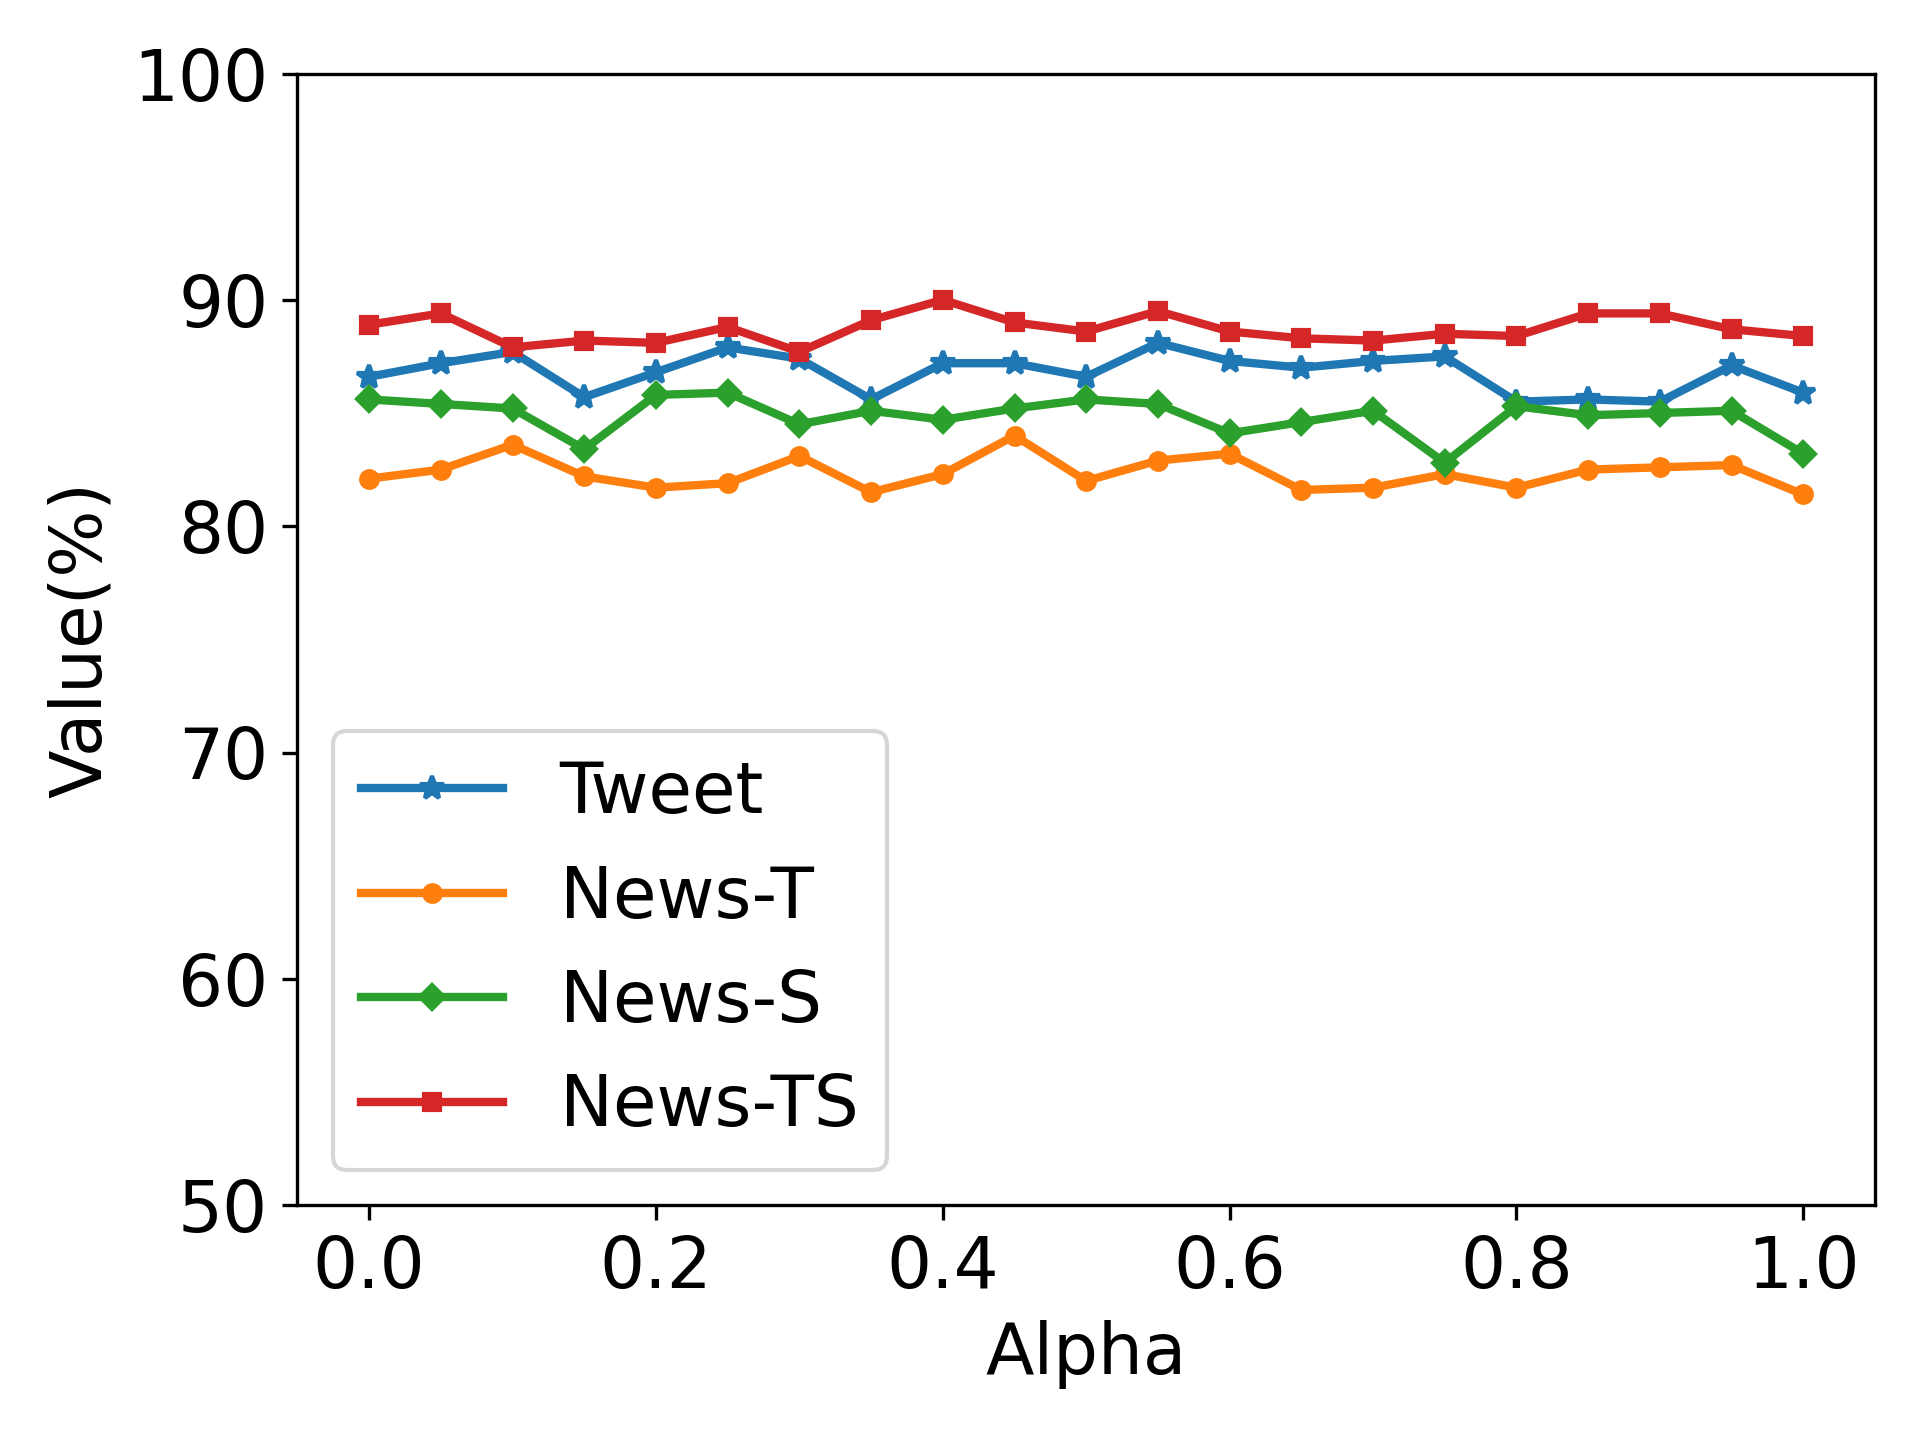
\includegraphics[width=0.98\textwidth]{figure/ACC_alpha.png}}
\centerline{(a) ACC}
\end{minipage}
\begin{minipage}{0.49\linewidth}
\centerline{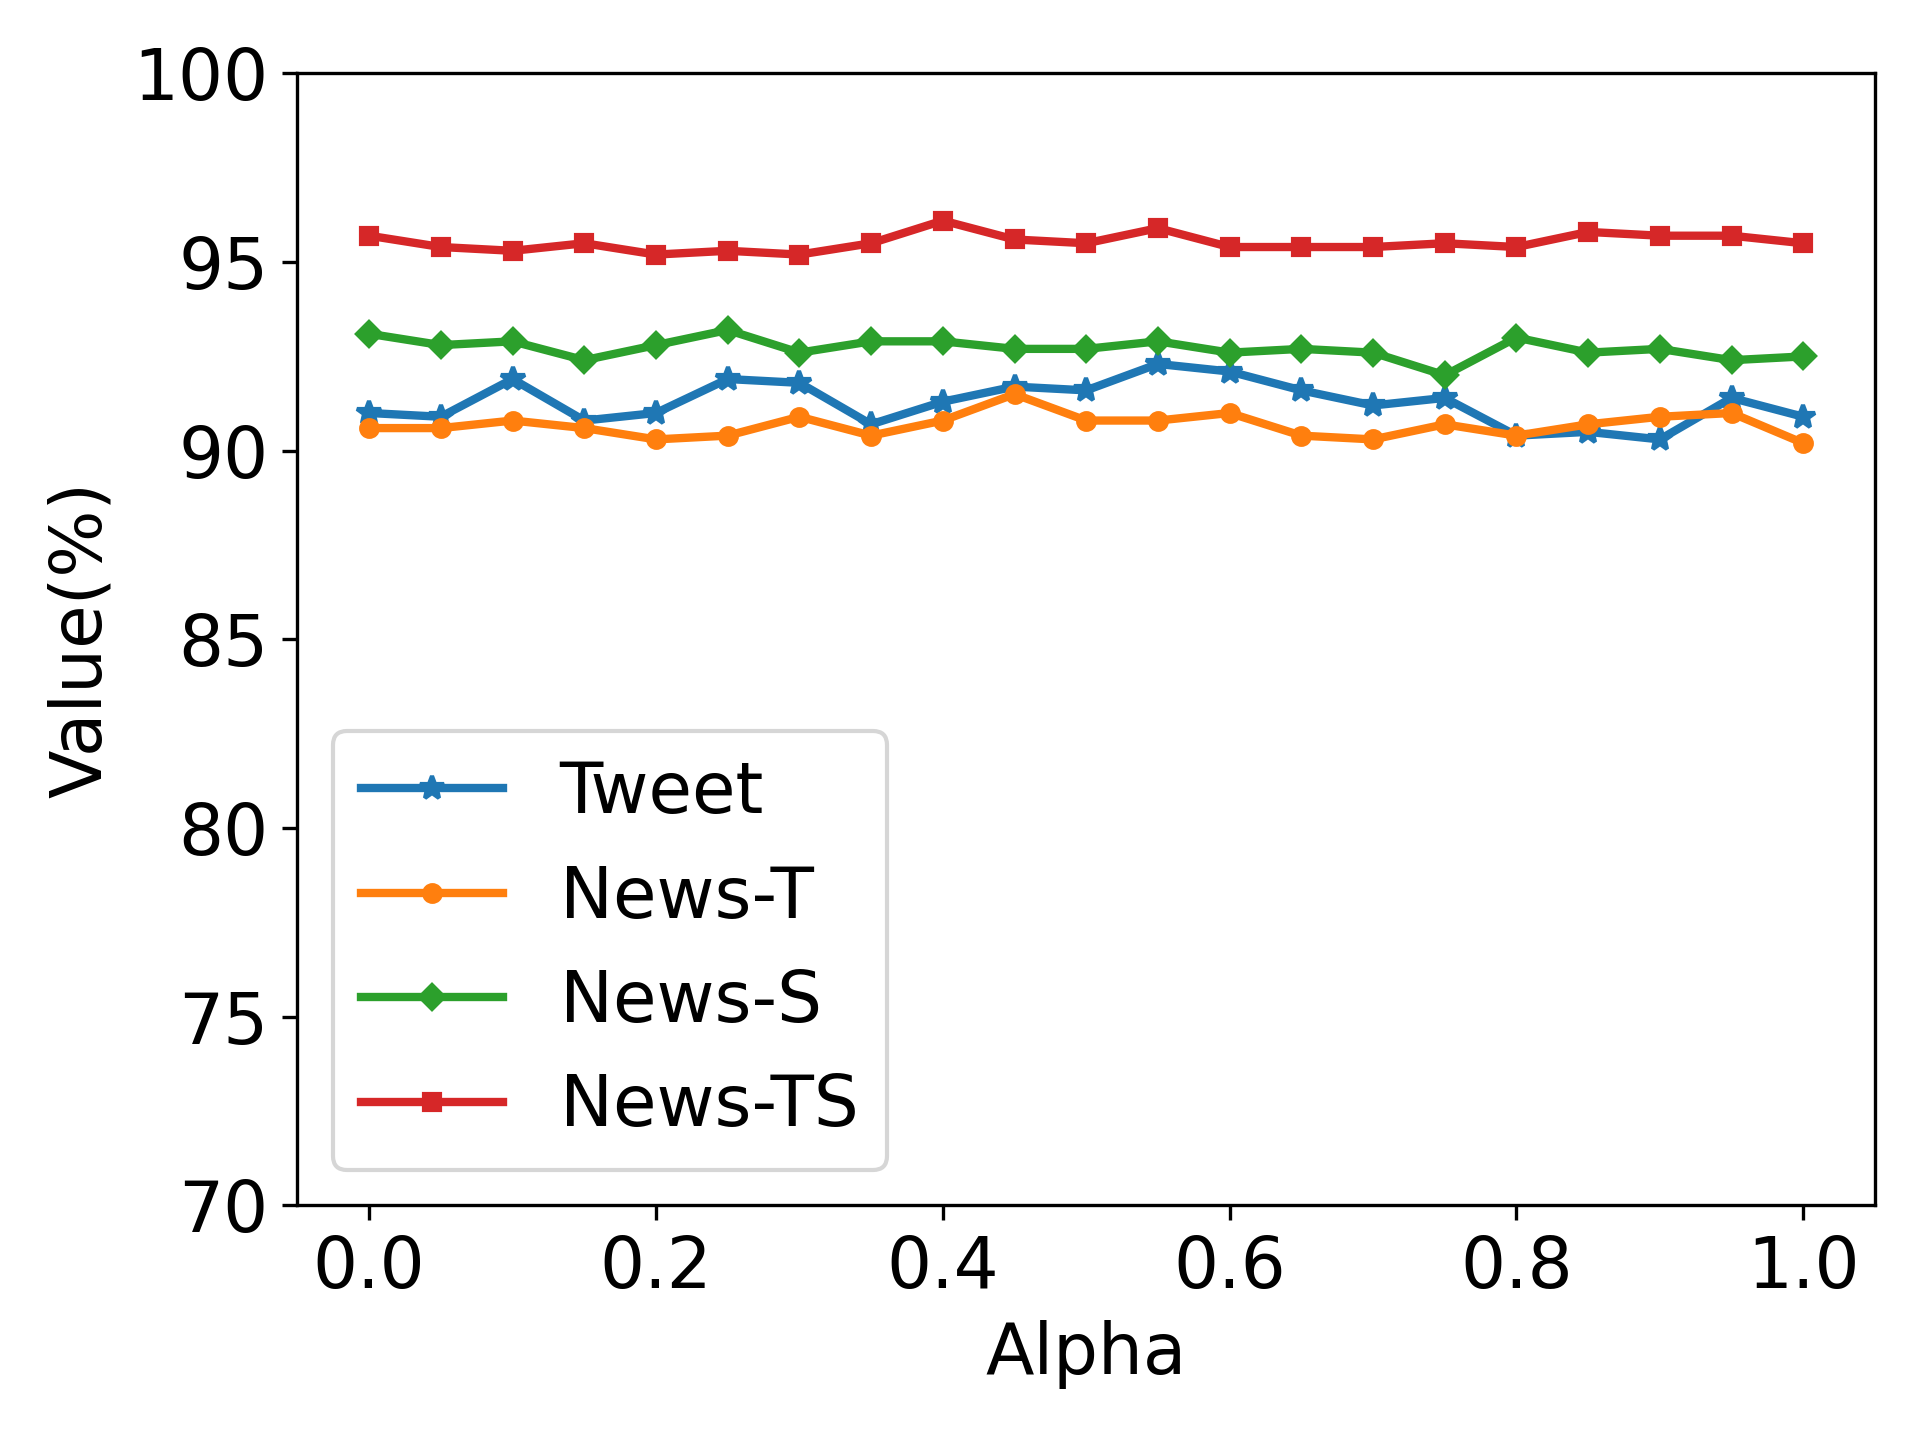
\includegraphics[width=0.98\textwidth]{figure/NMI_alpha.png}}
\centerline{(b) NMI}
\end{minipage}
\caption{The performance of \sysname{} with different values of $\alpha$ on four datasets.}
\label{alpha_analysis}
\end{figure}
In this section, we primarily present the hyper-parameter analysis of the improved \sysname{}, as it achieves the best performance.

1) \textbf{Influence of $\boldsymbol{\alpha}$:}
We investigate the impact of parameter $\alpha$ and vary the value of $\alpha$ from 0 to 1.0 with a step size of 0.05. The experimental results are presented in Figure~\ref{alpha_analysis}. As illustrated in the figures, we can see the performance of \sysname{} is stable with different values of $\alpha$.

We conduct experiments to investigate the performance of \sysname{} when $\alpha=0$, and find that \sysname{} almost does not result in clusters with only one document when $\alpha=0$. We should note that we can also speed up \sysname{} by setting $\alpha$ to zero. Because when $\alpha=0$, we can just discard clusters that get empty as they will never be chosen again. Futhermore, we should note that Equation~\eqref{eq:dpm3.4.7} cannot be derived from DMM when $\alpha=0$, because $\alpha$ is the parameter of the Dirichlet distribution in DMM and must be larger than zero.

\begin{figure}[!t]
\centering
\begin{minipage}{0.49\linewidth}
% \centerline{Positive Sample Pairs}
\centerline{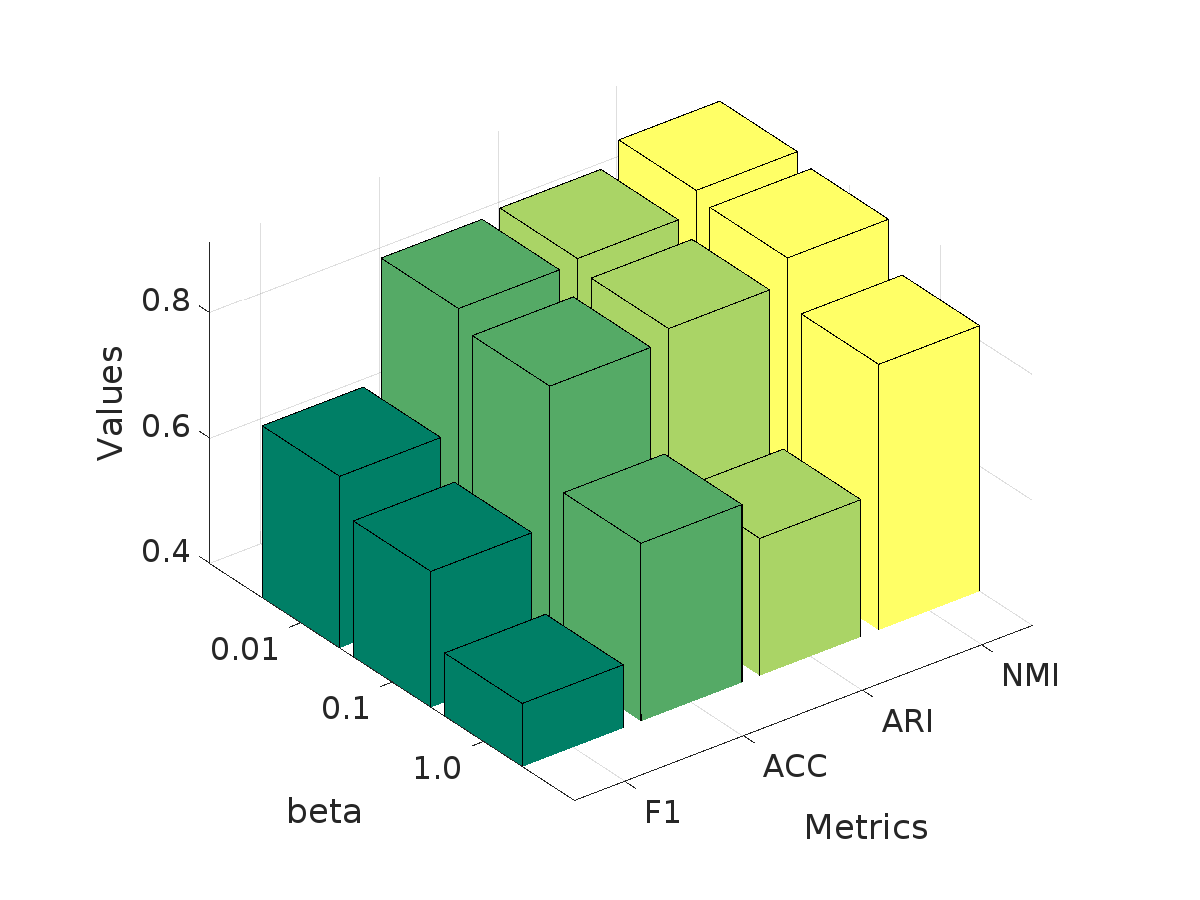
\includegraphics[width=0.98\textwidth]{figure/Tweet_HP.png}}
\centerline{(a) Tweet}
\centerline{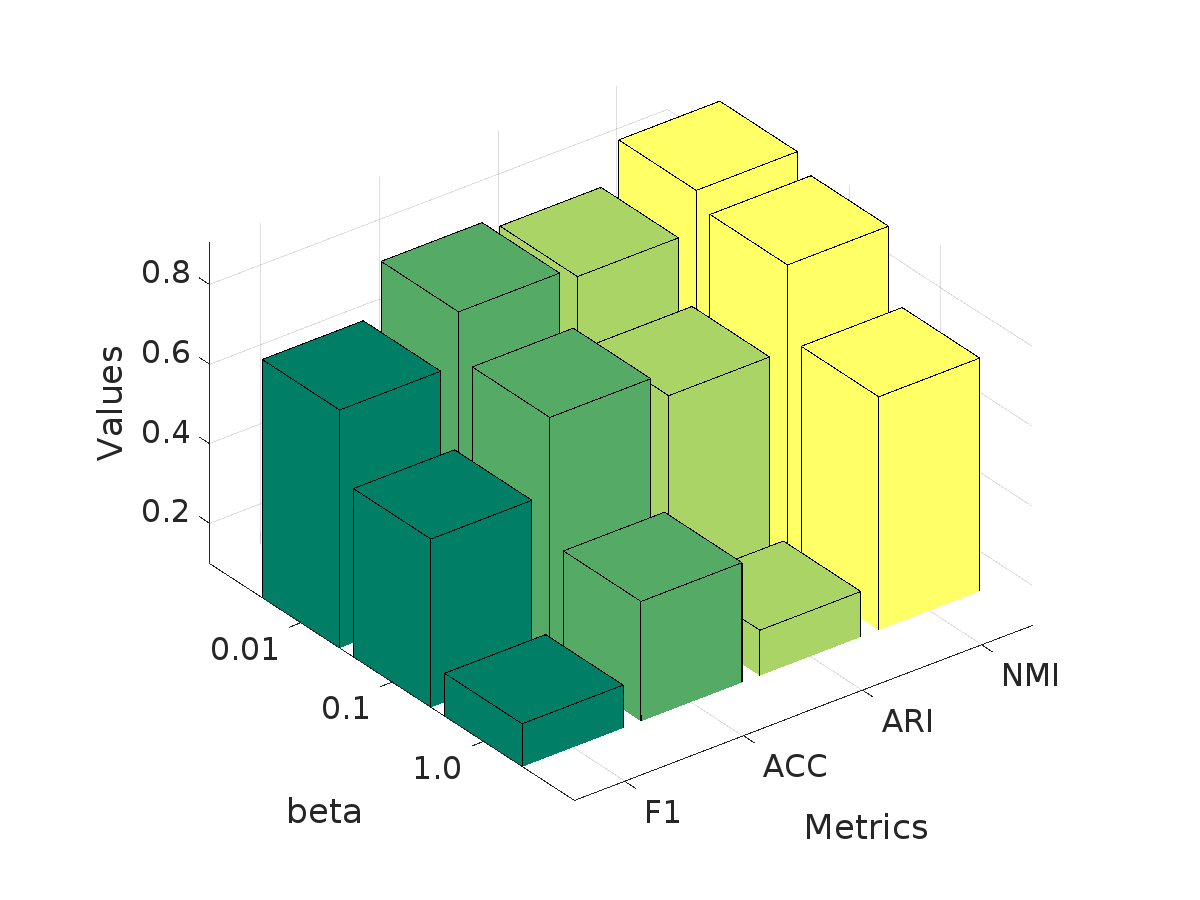
\includegraphics[width=0.98\textwidth]{figure/T_HP.png}}
\centerline{(c) News-T}
\end{minipage}
\begin{minipage}{0.49\linewidth}
% \centerline{Negative Sample Pairs}
\centerline{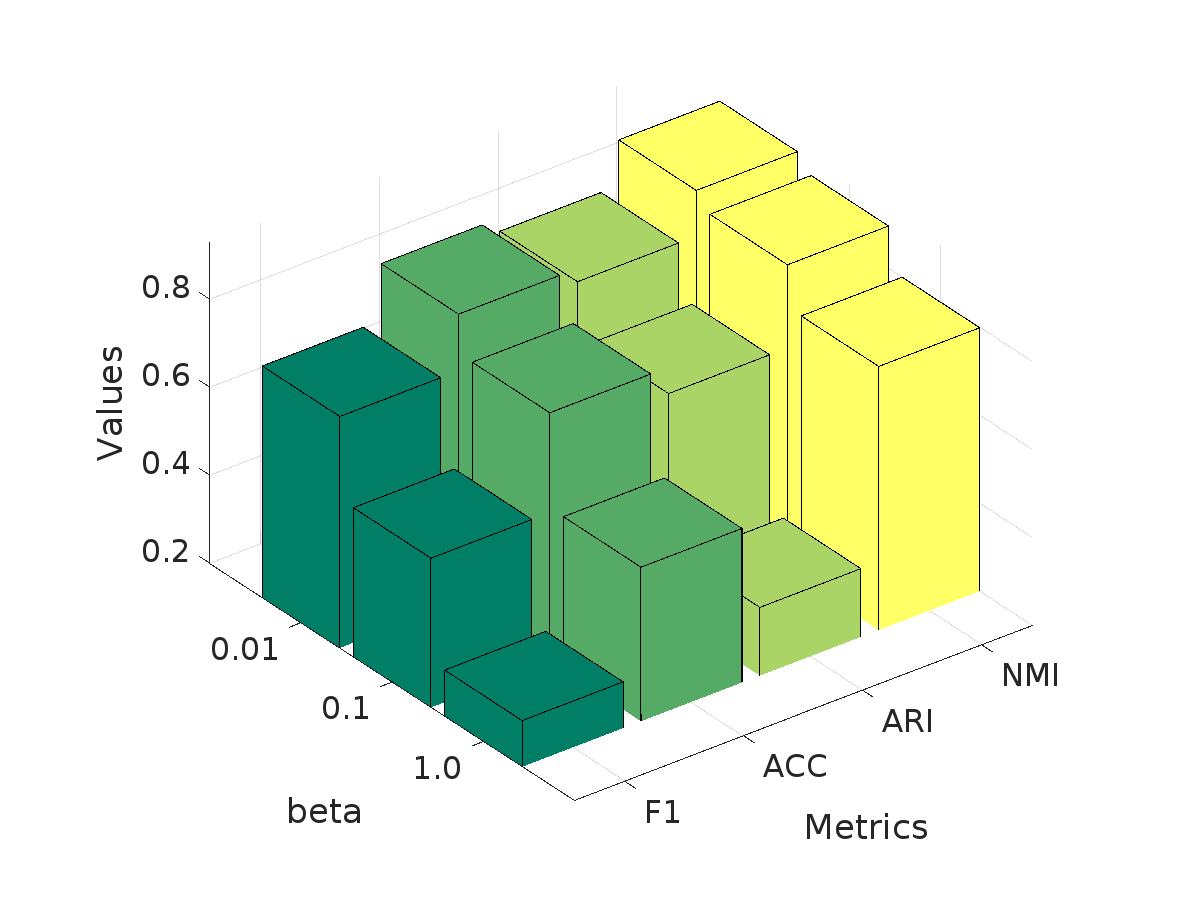
\includegraphics[width=0.98\textwidth]{figure/S_HP.png}}
\centerline{(b) News-S}
\centerline{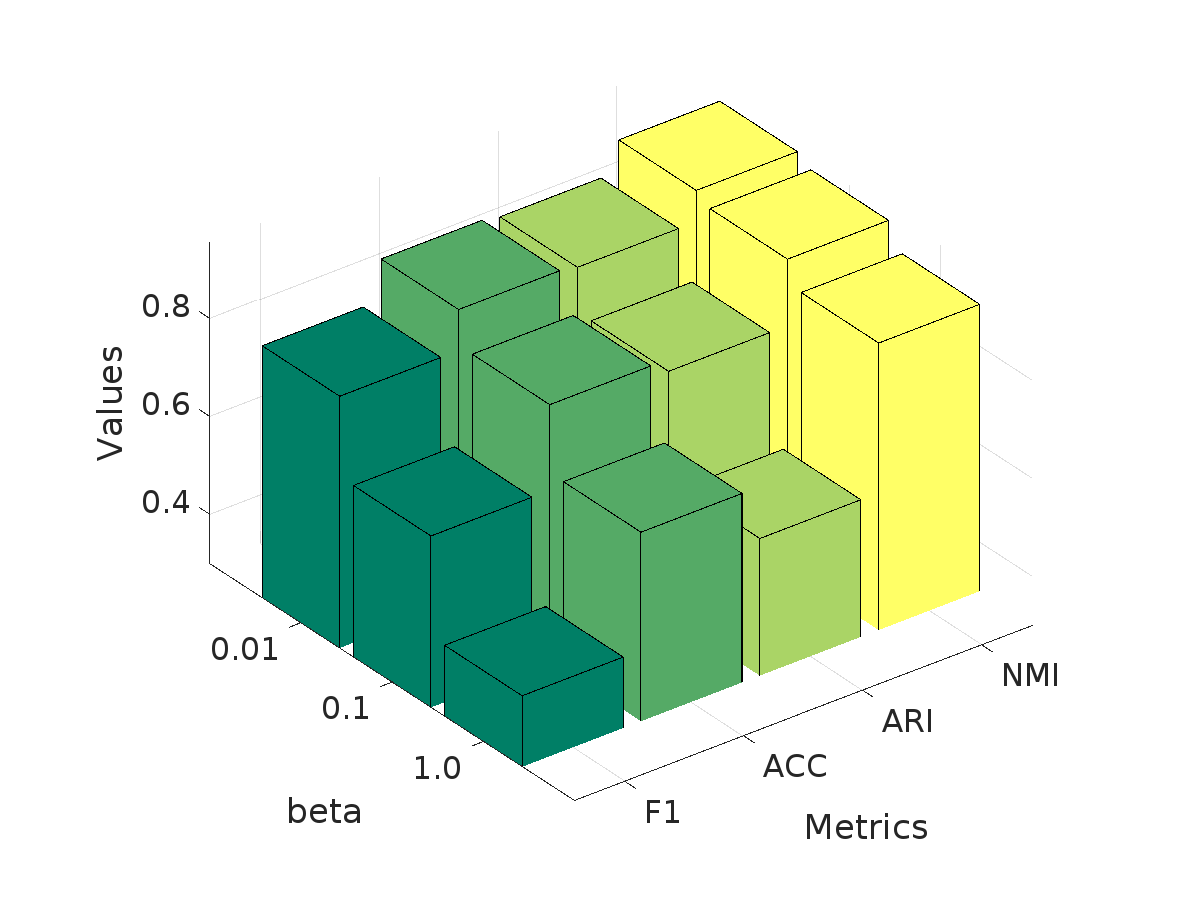
\includegraphics[width=0.98\textwidth]{figure/TS_HP.png}}
\centerline{(d) News-TS}
\end{minipage}
\caption{Hyper-parameter analysis for $\beta$.}
\label{hyper_parameters_beta}
\end{figure}

2) \textbf{Influence of $\boldsymbol{\beta}$:}
We try to investigate the influence of $\beta$ to the number of clusters found by \sysname{} and the performance of \sysname{}.

% \begin{table}[ht]
% \centering
% \caption{The accuracy and NMI of \sysname{} with different $\beta$ values used in adaptive clustering initialization.}
% \renewcommand{\arraystretch}{1.3} % 调整行间距
% \begin{tabular}{c|cccccc}
% \textbf{beta ($\beta$)}  & 0    & 1e-5 & 1e-4 & 0.001 & 0.01 & 0.1   \\ \hline
% \textbf{Accuracy (\%)}   & fail & 89.6 & 89.5 & 89.5  & 88.9 & 82.4  \\
% \textbf{NMI (\%)}        & fail & 95.8 & 95.9 & 96.0  & 95.7 & 93.1  \\
% \multicolumn{7}{c}{(a) News-TS} \\
% \end{tabular}
% % \vspace{10mm}
% \begin{tabular}{c|cccccc}
% \textbf{beta ($\beta$)}  & 0    & 1e-5 & 1e-4 & 0.001 & 0.01 & 0.1   \\ \hline
% \textbf{Accuracy (\%)}   & fail & 82.5 & 81.3 & 83.8  & 85.5 & 76.4  \\
% \textbf{NMI (\%)}        & fail & 92.3 & 91.9 & 92.6  & 92.9 & 89.2  \\
% \multicolumn{7}{c}{(b) News-S} \\
% \end{tabular}
% \label{beta_analysis}
% \end{table}

\begin{table}[ht]
\centering
\caption{The accuracy and NMI of \sysname{} with different $\beta$ values used in adaptive clustering initialization.}
\renewcommand{\arraystretch}{1.3} % 调整行间距
\setlength{\tabcolsep}{6pt} % 调整列间距
\begin{tabular}{c|c|cccccc}
\toprule
\textbf{Dataset} & \textbf{beta ($\beta$)} & 0 & 1e-5 & 1e-4 & 0.001 & 0.01 & 0.1 \\ 
\midrule
\multirow{2}{*}{News-TS} 
& Accuracy (\%) & fail & 89.6 & 89.5 & 89.5 & 88.9 & 82.4 \\
& NMI (\%) & fail & 95.8 & 95.9 & 96.0 & 95.7 & 93.1 \\
\midrule
\multirow{2}{*}{News-S}  
& Accuracy (\%) & fail & 82.5 & 81.3 & 83.8 & 85.5 & 76.4 \\
& NMI (\%) & fail & 92.3 & 91.9 & 92.6 & 92.9 & 89.2 \\
\bottomrule
\end{tabular}
\label{beta_analysis}
\end{table}

As shown in Table~\ref{beta_analysis}, in the News-TS dataset, our model performs reasonably well when $\beta$ is in the range of $1 \times 10^{-5}$ to 0.01. However, in the News-S dataset, as $\beta$ decreases, the granularity becomes excessively fine, leading to ineffective cluster merging and a decline in clustering performance. Additionally, when $\beta$ is too large (e.g., 0.1), the accuracy and NMI decrease significantly. At the extreme case of $\beta = 0$, as discussed in Section~\ref{sec:disAlpahAndBeta}, the model cannot be trained. Figure~\ref{S_deep_beta} provides a clearer illustration of how NMI and the number of clusters change with $\beta$ on the News-S dataset. These results validate our approach. By choosing $\beta = 0.01$, we achieve sufficiently fine-grained clusters that capture subtle local patterns while also benefiting from effective cluster merging for improved clustering performance.

\begin{figure}[t]
\centering
\begin{minipage}{0.98\linewidth}
\centerline{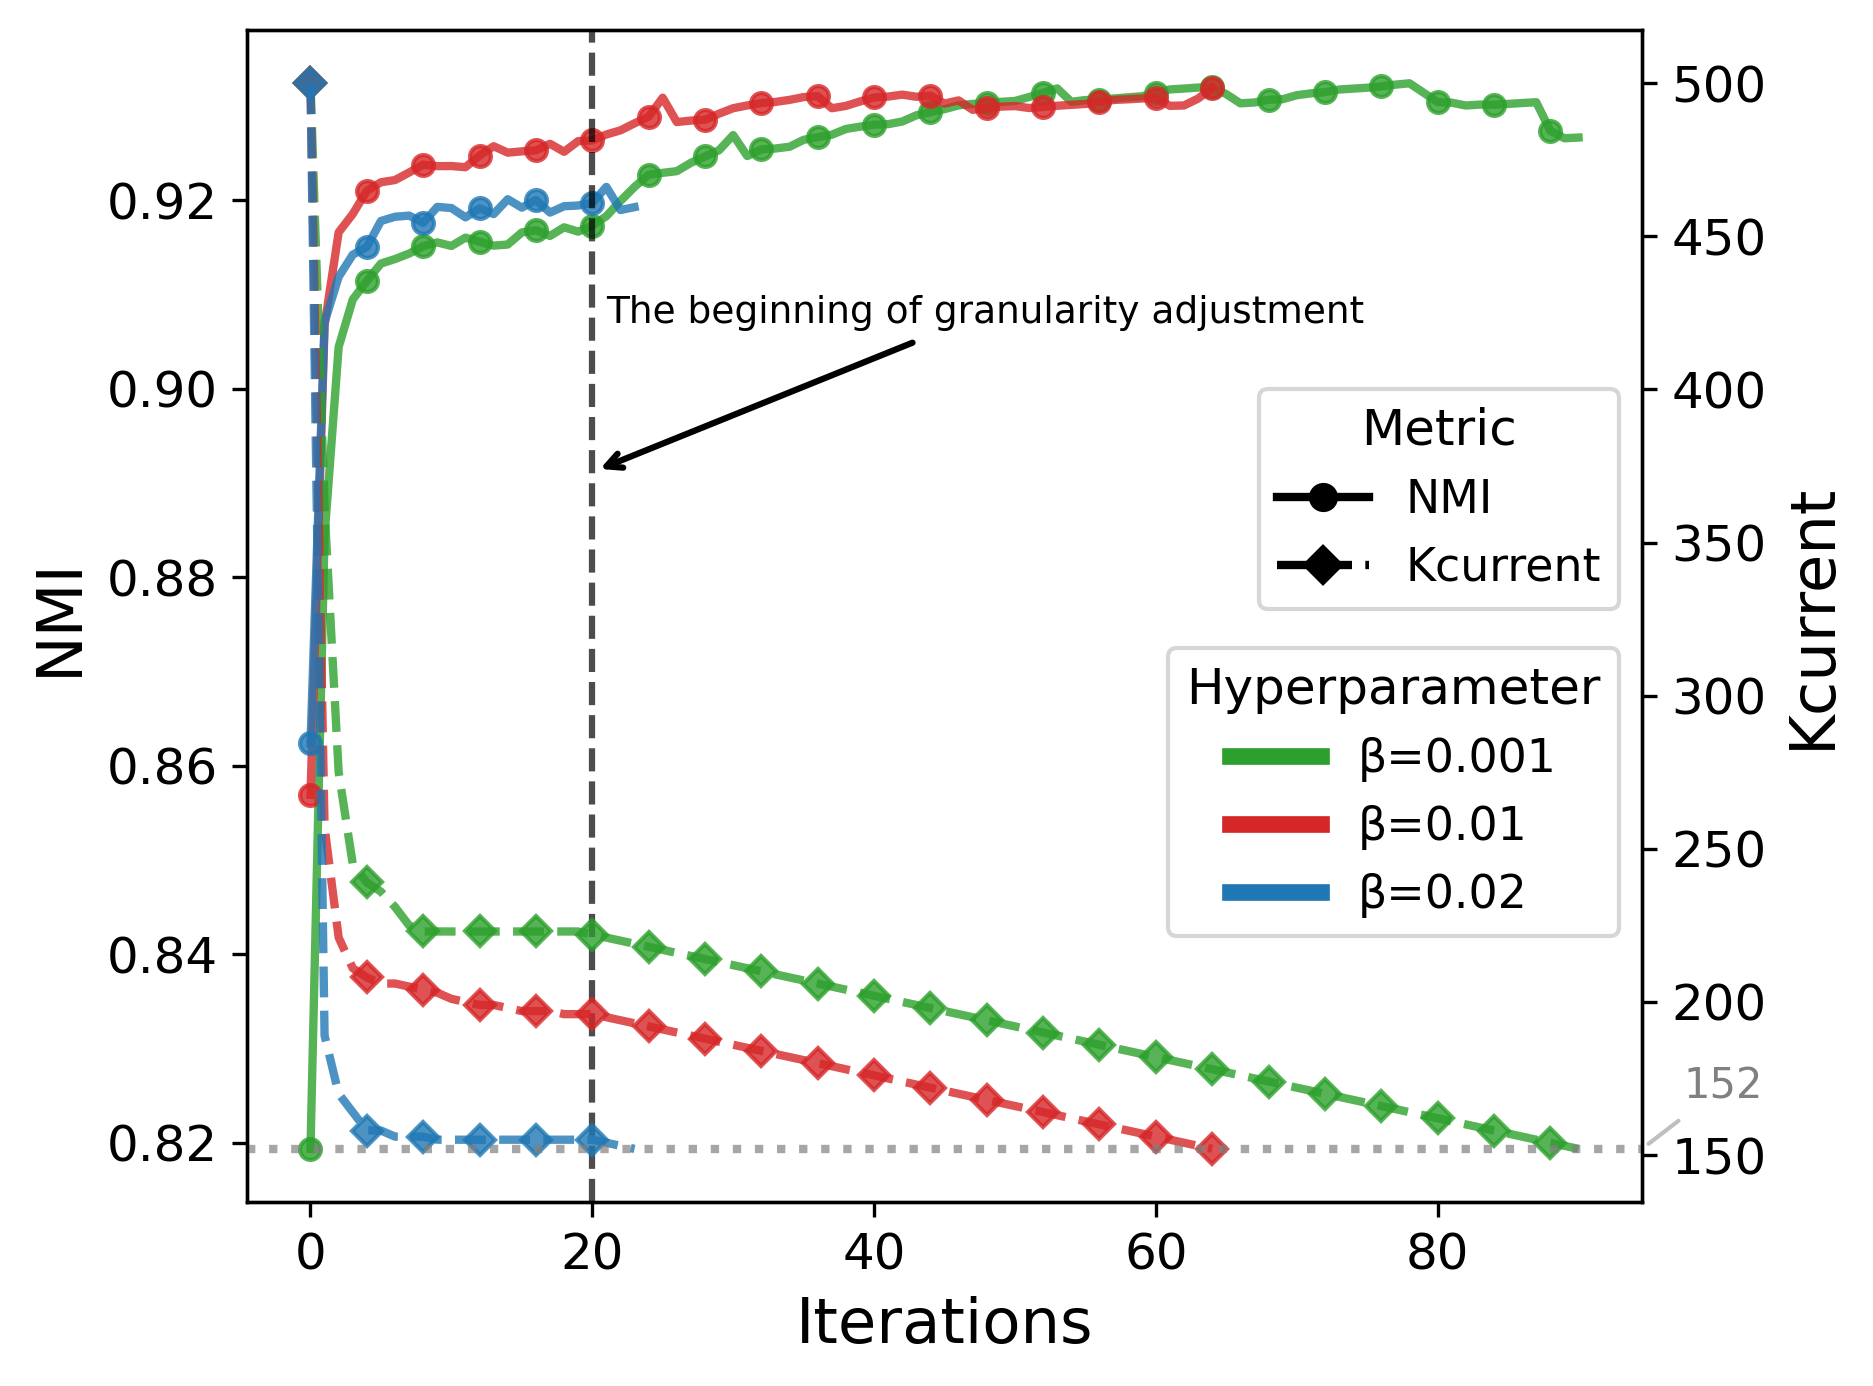
\includegraphics[width=0.98\textwidth]{figure/S_deep_beta.png}}
\end{minipage}
\caption{The variations in NMI and the number of clusters on the News-S dataset.}
\label{S_deep_beta}
\end{figure}

% Figure \ref{fig:GSDMMPredKBeta} shows the number of clusters found by GSDMM with different values of $\beta$ on the four datasets. From Figure \ref{fig:GSDMMPredKBeta}, we can see the number of clusters found by GSDMM drops when we enlarge $\beta$.
% This is because $\beta$ is in the second part of Equation \ref{eq:con2} which relates to Rule 2 of MGP (Choose a table whose students share similar interests with him). When $\beta$ is small, the probability of a student choosing a table is more sensitive to $n_{z,\neg{d}}^{w}$ (the number of occurrences of word $w$ in cluster $z$). In other words, GSDMM gives more emphasis on the student's interests when $\beta$ is small, and the students will have a larger probability to choose a table based on their interests rather than the popularity of tables.  As a result, GSDMM will result in more non-empty tables (clusters) when $\beta$ is small. Similarly, when $\beta$ is large, GSDMM will result in fewer non-empty tables.
